\subsection{Áp dụng dataset cho bài toán}
Kiến trúc giải thuật mà nhóm sẽ sử dụng  gồm hai mô hình được xếp chồng lên nhau. Mô hình thứ nhất thực hiện nhiệm vụ xác định vị trí biển báo giao thông đang ở đâu trong bức ảnh được camera của xe ghi lại, có rất nhiều loại biển báo và sẽ được chia thành bốn loại lớn là:
\begin{itemize}
    \item Biến cấm: bao gồm các biển báo giao thông có hình tròn, nền trắng và viền đỏ. VD: giới hạn tốc độ, ... 
    \item Biển nguy hiểm: bao gồm các biển báo giao thông có hình tam giác, nền trắng và viền đỏ. VD: ngã tư, đường trơn trượt, ... 
    \item Biển bắt buộc : bao gồm các biển báo giao thông có hình tròn và nền màu xanh. VD: rẽ trái, rẽ phải, đi thẳng, ... 
    \item Các loại còn lại: bao gồm các biển báo giao thông không thuộc các danh mục trước đó. VD: đường ưu tiên, dừng lại, ... 
\end{itemize}
Sau khi dã xác định được vị trí của biển báo, hình ảnh sẽ được thu gọn lại vào bounding box của biển báo, sử dụng output của mô hình thứ nhất, điều chỉnh ảnh về kích thước 32x32 làm input cho mô hình thứ hai sử dụng mạng CNN và deep learning như đã đề cập ở trên để phân loại cụ thể đó là biển báo gì trong 43 lớp đã được xác định từ trước của bộ dataset. Như vậy, bằng việc sử dụng 2 lớp mô hình chồng lên nhau ta có thể giải quyết được vấn đề đặt ra.\\
Ta có thể tóm gọn lại kiến trúc cho bài toán phát hiện biển báo như sau:
\begin{figure}[htp]
    \centering
    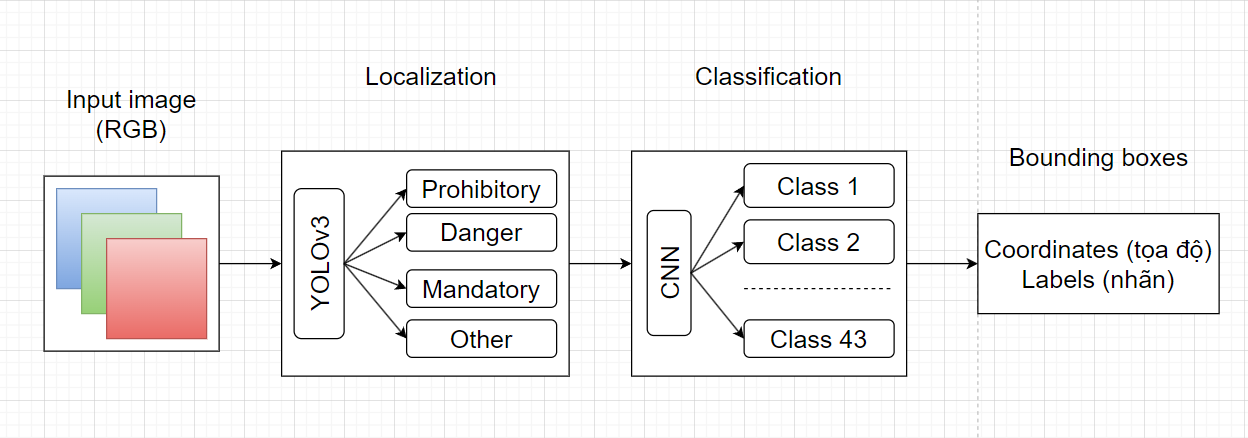
\includegraphics[width=0.8\textwidth]{images/2c-sign/sign-sys.png}
    \caption{Giải thuật}
    \label{fig:algo}
\end{figure}

\noindent Quay trở lại, ta đã đề cập là sẽ sử dụng hai bộ dữ liệu có sẵn là bộ biển báo giao thông của Đức GTSDB và GTSRB. Mô hình thứ nhất được huấn luyện trên bộ dữ liệu GTSDB (German Traffic Sign Detection Benchmark) gồm 900 bức ảnh đầu vào dạng RGB. Bộ dữ liệu bao gồm cả những hình ảnh không có biển báo giao thông để sử dụng trong quá trình huấn luyện. Tuy nhiên, quyết định đã được đưa ra để loại bỏ những hình ảnh này. Bộ dữ liệu kết quả đã được chia thành các tập con để huấn luyện và kiểm tra. \\
\newline
Nhãn cho các bounding box của từng hình ảnh được lưu trong 1 file txt như sau:

\begin{lstlisting}
00001.ppm;983;388;1024;432;40
00001.ppm;386;494;442;552;38
00001.ppm;973;335;1031;390;13
\end{lstlisting}
Thông số đầu tiên là tên bức ảnh, được lưu dưới dạng .ppm. Năm thông số tiếp theo lần lượt là: tọa độ góc trái, tọa độ góc phải, lớp (biển báo thuộc về lớp bao nhiêu trong 43 lớp đã xác định trước). Ví dụ:
\begin{lstlisting}[language = Python]
0 = speed limit 20 (prohibitory)
...
9 = no overtaking (prohibitory)
...
14 = stop (other)
...
31 = animals (danger)
33 = go right (mandatory)
34 = go left (mandatory)

\end{lstlisting}
Đầu tiên ta cần chuyển tất cả thông số này về định dạng mà YOLO dùng để huân luyện: tọa độ tâm x, tọa độ tâm y, chiều rộng và chiều cao của đối tượng, đồng thời chuẩn hóa các thông số về đoạn [0,1]. Sử dụng công thức như sau:
\begin{equation*}
    \begin{aligned}
        X_{centre} &= \frac{X_{min} + X_{max} }{2} \cdot \frac{1}{w}\\
        Y_{centre} &= \frac{Y_{min} + Y_{max} }{2} \cdot \frac{1}{h}\\
        width &= \frac{X_{max} - X_{min} }{2} \cdot \frac{1}{w}\\
        height &= \frac{Y_{max} - Y_{min} }{2} \cdot \frac{1}{h}\\
    \end{aligned}
\end{equation*}
Ta thu được các file .ppm được chuyển sang định dạng .jpg, với mỗi ảnh sẽ là một file.txt chứa các thông số được chuẩn hóa cho từng bounding box của biển báo:
\begin{figure}[htbp]
    \centering
    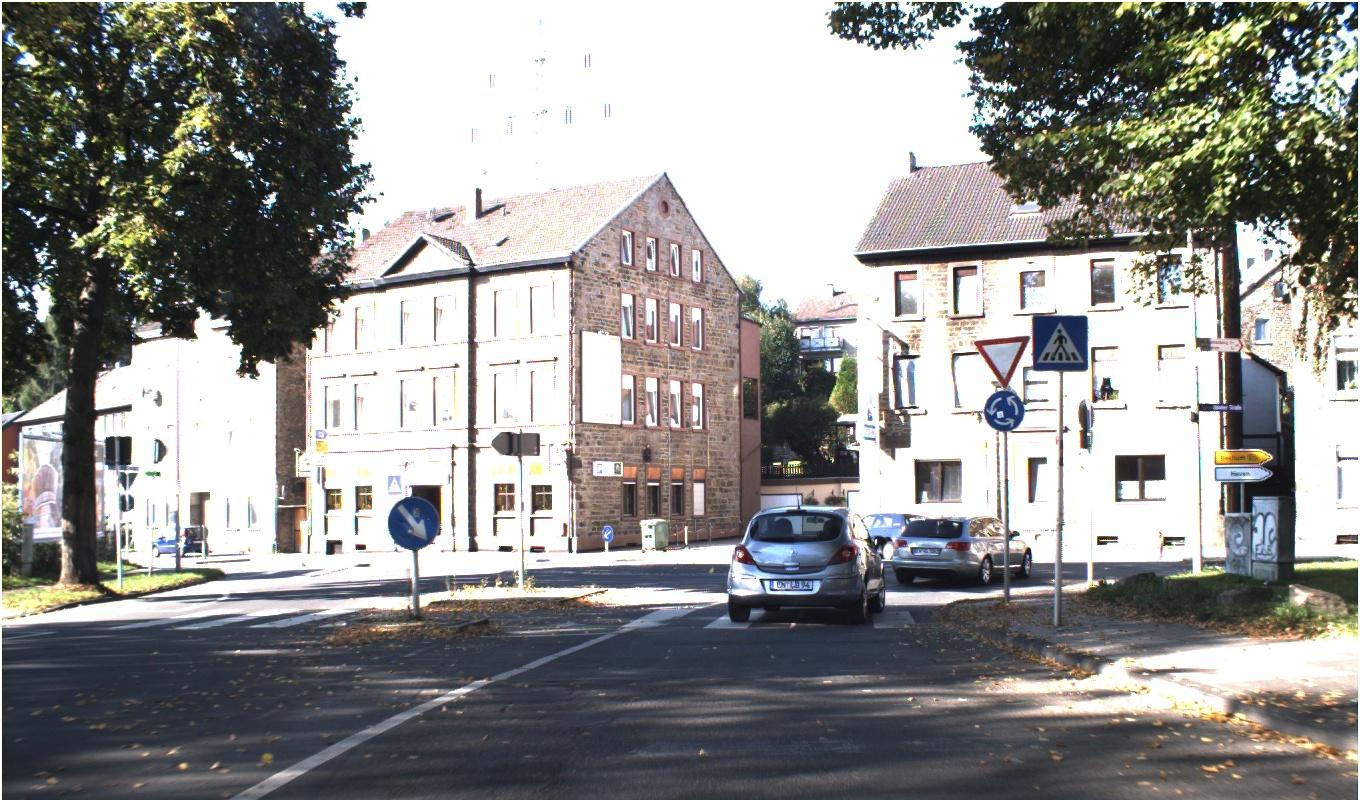
\includegraphics[width = 0.6\textwidth]{images/2c-sign/00001.jpg}
    \caption{Ảnh dataset}
\end{figure}
\begin{lstlisting}[language = Python]
#class X Y W H
2 0.7378676470588236 0.5125 0.030147058823529412 0.055
2 0.3044117647058823 0.65375 0.041176470588235294 0.0725
3 0.736764705882353 0.453125 0.04264705882352941 0.06875
\end{lstlisting}
Lúc này ta đã chuẩn bị đầy đủ dữ liệu để cho ra mô hình thứ nhất sử dụng YOLOv3.

\noindent Sau khi training xong và thu được file .weight với kết quả tốt nhất, ta tiếp tục đến với huấn luyện mô hình thứ hai - phân loại biển báo. \\
\newline 
Mô hình thứ hai được huấn luyện trên GTSRB với tổng cộng 66,000 hình ảnh RGB có dạng 32x32x3, gồm 43 loại biển báo mà ta đã đề cập đến ở phía trên. Ta có thể xem qua số lượng của từng loại biển báo như sau:
\newpage
\begin{figure}[htbp]
    \centering
    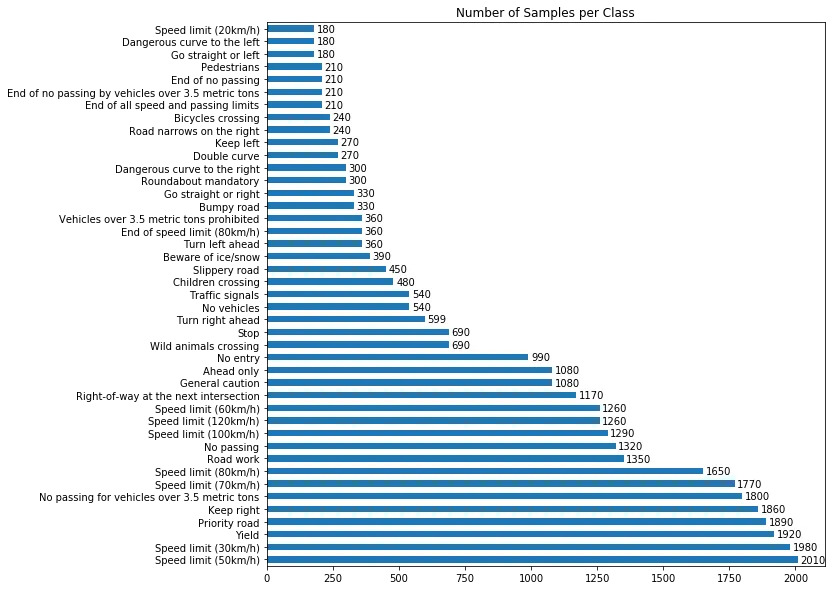
\includegraphics[width = 0.7\textwidth]{images/2c-sign/overall.jpg}
    \caption{Tổng quan GTSRB}
    \label{fig:overall}
\end{figure}

\noindent Tập dữ liệu này cũng sẽ chia thành nhiều phần với tý lệ nhất định cho ba mục đích gồm huấn luyện, kiểm tra và kiểm thử mô hình. Dựa vào \hyperlink{fig:overall}{\textcolor{blue}{hình}} trên ta thấy có sự chênh lệch không nhỏ giữa các biển báo khác nhau, vì thế trước khi huấn luyện cần làm thêm một bước là tăng cường dữ liệu:
\begin{lstlisting}[language = Python]
aug = ImageDataGenerator(rotation_range=0.18, 
                            zoom_range=0.15, 
                            width_shift_range=0.2, height_shift_range=0.2, 
                            horizontal_flip=True)
\end{lstlisting}

Sau khi huấn luyện cho mô hình thứ hai xong và nhận được kết quả như mong muốn, ta lưu model lại với định dạng .h5 để tiếp tục sử dụng. Dựa trên giải thuật đã trình bày trong \hyperlink{fig:algo}{\textcolor{blue}{hình}} ta cần tiền xử lí output của mô hình thứ nhất trước khi đưa nó vào làm input cho mô hình dự đoán thứ hai:
\begin{enumerate}
    \item \textbf{Gray-scale:} \\
    Do ảnh ban đầu có định dạng là RGB là một tập hợp gồm các điểm, mà mỗi điểm là bộ 3 màu red, green và blue, như vậy sẽ chứa các thông tin không cần thiết. Việc gray-scale giúp cho ta giảm bớt số lượng thông tin dư thừa, đồng thời phù hợp với model chúng ta train (lúc train model ta sử dụng ảnh gray-scale, nên khi ta predict ta cũng phải sử dụng ảnh gray-scale)
    \item \textbf{Sửa kích thước thành 32x32}\\
    Tùy thuộc vào vị trí đứng của xe, mà biển báo nhìn thấy được trong hình sẽ to hay nhỏ,
nên ta cần resize lại về cùng 1 kích thước. Khi đó ta mới có thể đem vào model.predict.
    \item \textbf{Local Histogram Equalization}\\
    Đây là phương pháp tăng độ tương phản cho ảnh khi ở dạng gray-scale. Nhờ vào phương
pháp này, ta có thể tăng độ chính xác khi predict.
\end{enumerate}
Về các biển báo cần nhận diện, trong chủ đề lần này, nhóm đã đề ra 1 số yêu cầu theo thứ tự ưu tiên để từ đó quyết định rằng tập dữ liệu cần thiết để giữ nguyên hay thay đổi số lượng của tập dữ liệu:
\begin{itemize}
    \item Tốc độ xử lý thời gian thực (Real-time processing)
    \item Độ chính xác cao (High precision)
\end{itemize}
Dựa trên hai tiêu chí này, nên trong quy mô của đồ án lần này model thứ hai sẽ bị lược bỏ bớt biển báo không cần thiết trong việc mô phỏng cũng như chạy kiểm thử, đồng thời chỉnh sửa một chút ở mô hình mạng CNN áp dụng để phù hợp hơn với số lượng mới cho tập dữ liệu. Như vậy, các biển báo nhóm sẽ sử dụng là:
\begin{itemize}
    \item Speed limit (60 km/h)
    \item Turn left ahead
    \item Turn right ahead
    \item Stop
\end{itemize}
Bằng cách này, tốc độ xử lí của xe trong mô phỏng cũng như hiệu suất dự đoán của mô hình sẽ nhanh và chính xác hơn. 
\subsubsection*{Kết quả thu được}
\newpage
\begin{itemize}
    \item \textbf{Speed limit (60 km/h)}
    \begin{figure}[htbp]
    \centering
    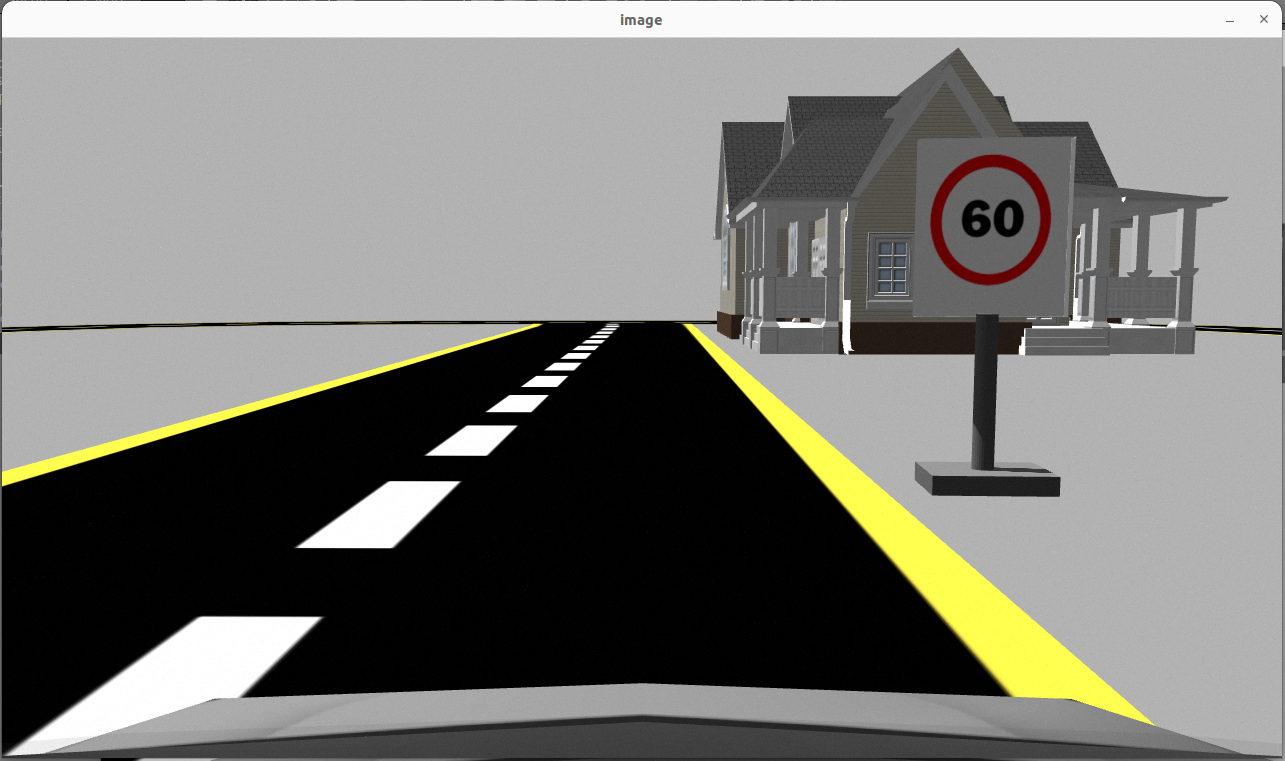
\includegraphics[width = 0.7\textwidth]{images/2c-sign/60-in.png}
    \caption{Input}
\end{figure}
    \begin{figure}[htbp]
    \centering
    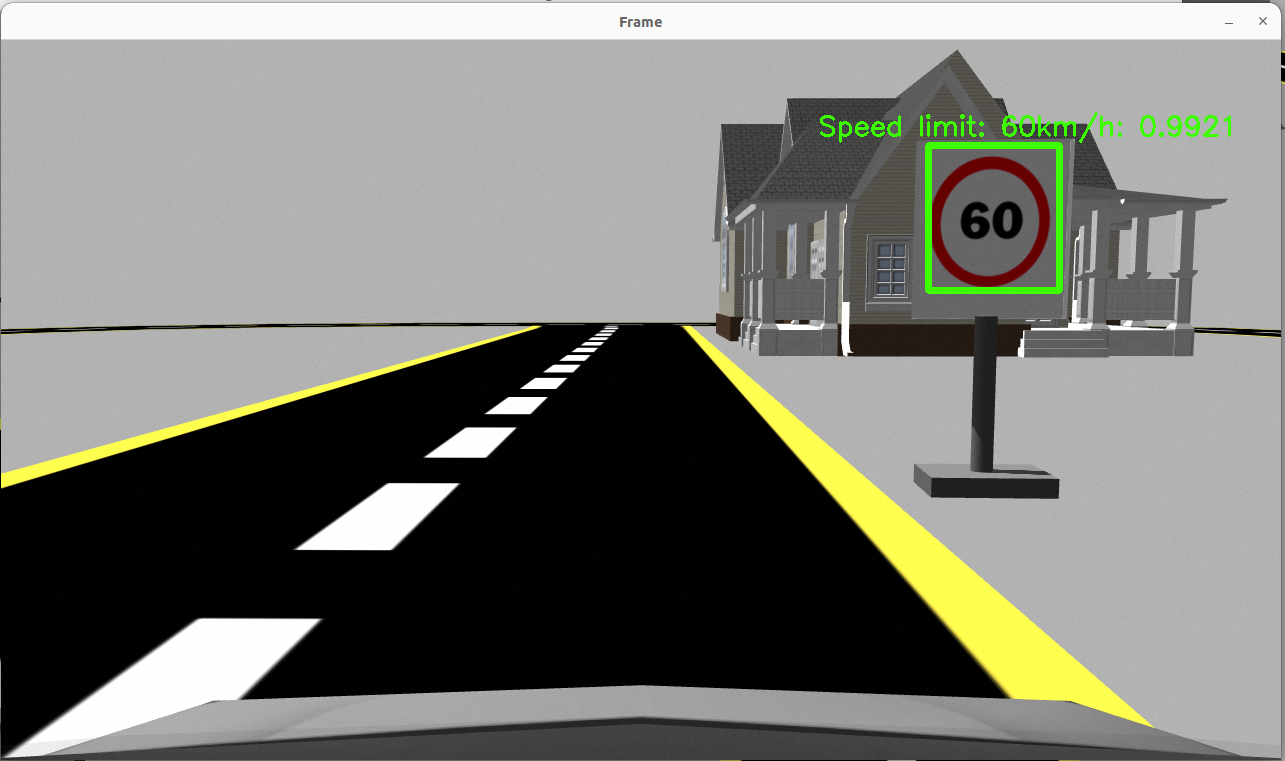
\includegraphics[width = 0.7\textwidth]{images/2c-sign/60-out.png}
    \caption{Output}
\end{figure}
\newpage
    \item \textbf{Turn left ahead}
    \begin{figure}[htbp]
    \centering
    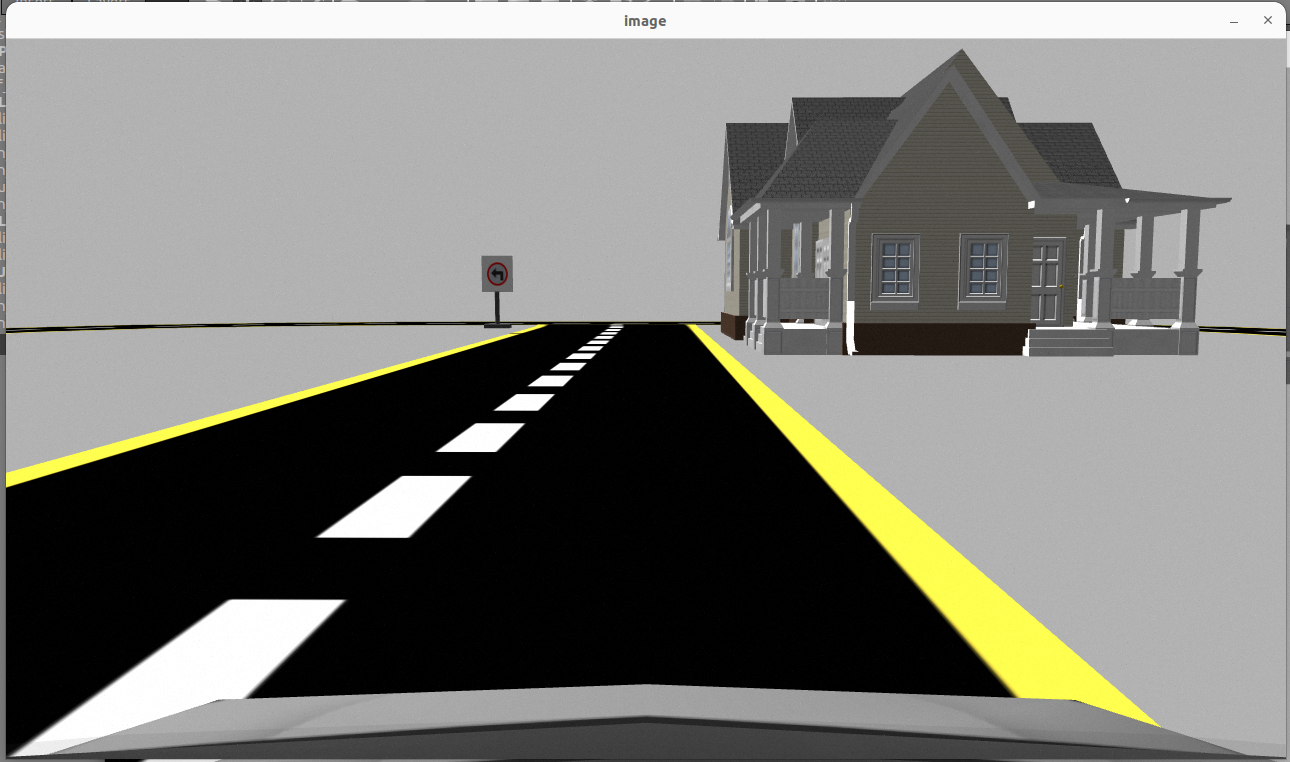
\includegraphics[width = 0.7\textwidth]{images/2c-sign/left-in.png}
    \caption{Input}
\end{figure}
    \begin{figure}[htbp]
    \centering
    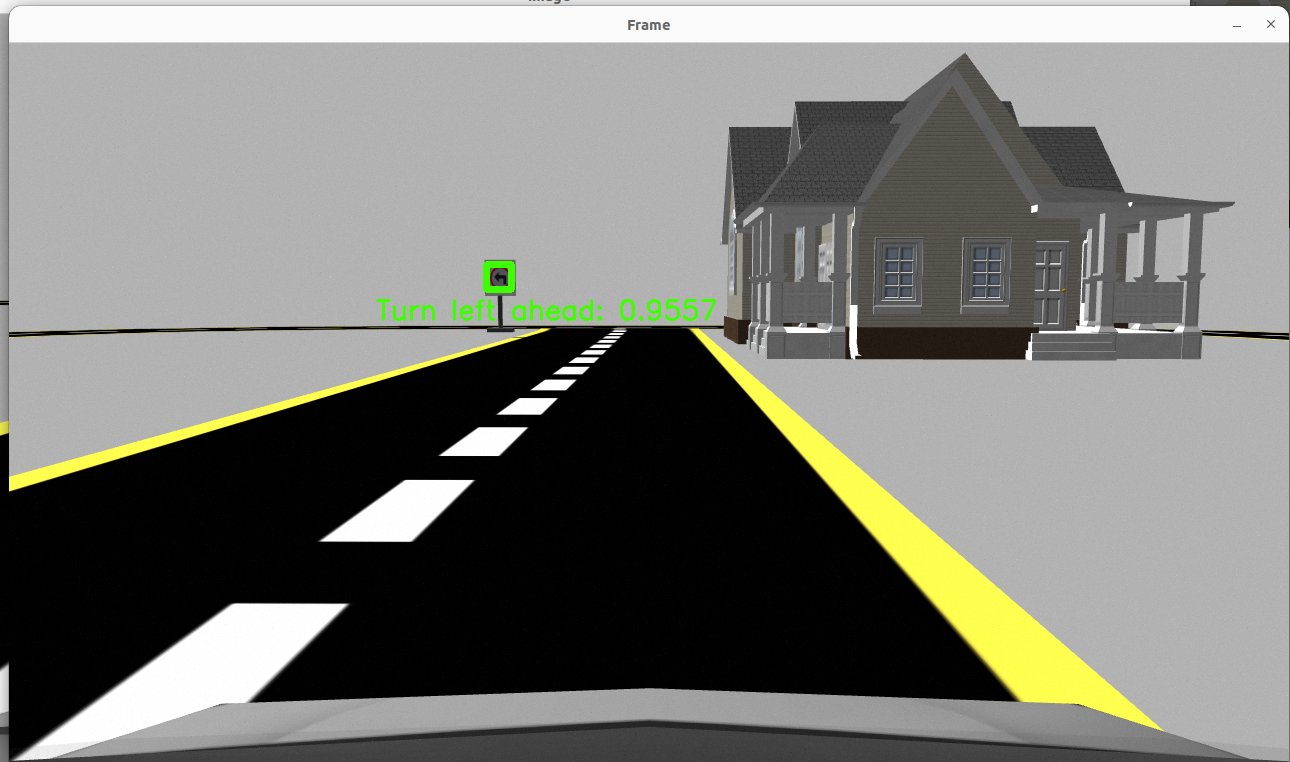
\includegraphics[width = 0.7\textwidth]{images/2c-sign/left-out.png}
    \caption{Output}
\end{figure}
\newpage
    \item \textbf{Stop}
    \begin{figure}[htbp]
    \centering
    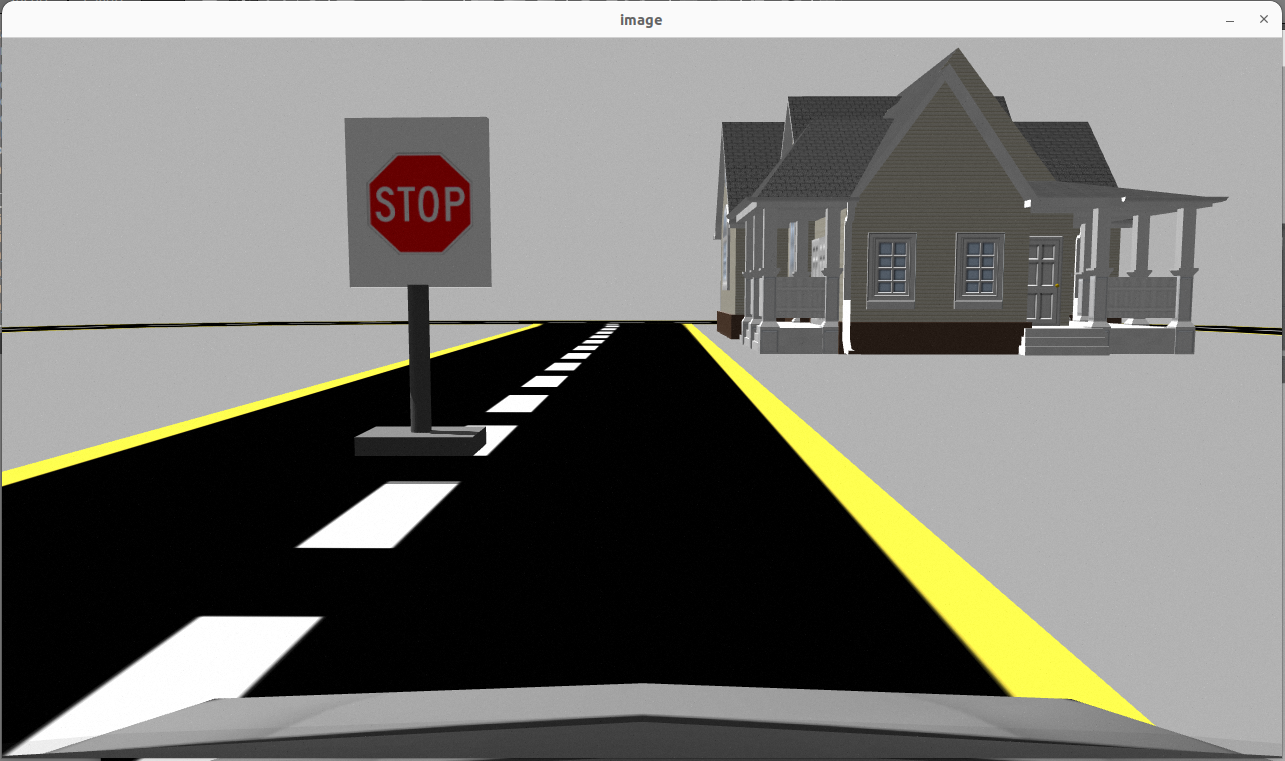
\includegraphics[width = 0.7\textwidth]{images/2c-sign/stop-in.png}
    \caption{Input}
\end{figure}
    \begin{figure}[htbp]
    \centering
    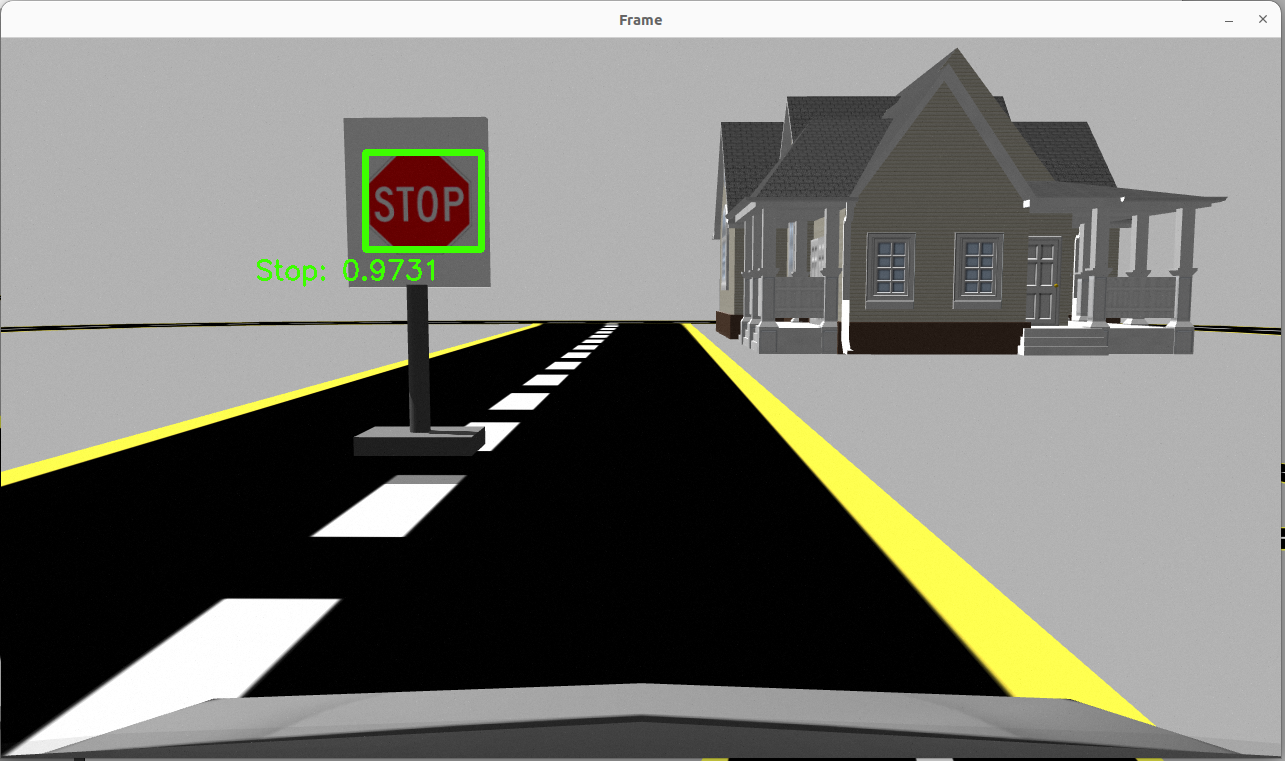
\includegraphics[width = 0.7\textwidth]{images/2c-sign/stop-out.png}
    \caption{Output}
\end{figure}
\end{itemize}
\newpage
